% Intended LaTeX compiler: xelatex
\documentclass[10pt, svgnames]{beamer}
\usepackage{graphicx}
\usepackage{longtable}
\usepackage{wrapfig}
\usepackage{rotating}
\usepackage[normalem]{ulem}
\usepackage{amsmath}
\usepackage{amssymb}
\usepackage{capt-of}
\usepackage{hyperref}
\usetheme{focus}
\author{Sappinandana Akamphon}
\date{\today}
\title{Intro to Material Behaviors}
\subtitle{ME 210: Mechanics of Materials}
\usepackage{booktabs}
\institute{Department of Mechanical Engineering, TSE}
\date{}
\usepackage{tikz-3dplot}
\usetikzlibrary{patterns,shapes,decorations,decorations.pathreplacing,decorations.pathmorphing}
\AtBeginSection[]{\begin{frame}{Outline}\tableofcontents[currentsection]\end{frame}}
\hypersetup{
 pdfauthor={Sappinandana Akamphon},
 pdftitle={Intro to Material Behaviors},
 pdfkeywords={},
 pdfsubject={},
 pdfcreator={Emacs 30.0.50 (Org mode 9.6)}, 
 pdflang={English}}
\begin{document}


\begin{frame}[label={sec:orgb021edc}]{\{\}}
\maketitle
\end{frame}

\begin{frame}[label={sec:org1caa009}]{A Little Intro}
\begin{itemize}
\item Name: Sappinandana Akamphon

\item Room: ENG 421/4

\item mail: sup@engr.tu.ac.th
\end{itemize}
\end{frame}

\begin{frame}[label={sec:orga5da805}]{Childhood}
\begin{itemize}
\item Born and raised in Khon Kaen, Thailand
\end{itemize}

\begin{center}
\includegraphics[height=0.8\textheight]{pictures/khonkaen.png}
\end{center}
\end{frame}

\begin{frame}[label={sec:orgc8fc742}]{Bachelor's Degree}
\begin{itemize}
\item Sc.B. Brown University, 2002
\end{itemize}

\begin{center}
\includegraphics[width=.9\linewidth]{pictures/brown.jpg}
\end{center}
\end{frame}

\begin{frame}[label={sec:orgd5825cc}]{Master and Doctoral}
\begin{itemize}
\item M.S. 2005, Ph.D. 2008, MIT
\end{itemize}

\begin{center}
\includegraphics[width=.9\linewidth]{pictures/mit.jpg}
\end{center}
\end{frame}

\begin{frame}[label={sec:orgcdc0e6c}]{Research Interests}
\begin{itemize}
\item Solar energy utilization

\item Water generation
\end{itemize}

\begin{center}
\includegraphics[width=.9\linewidth]{pictures/awg.jpg}
\end{center}
\end{frame}

\begin{frame}[label={sec:org3d71f2d}]{Material Behaviors}
\begin{itemize}
\item The study of material response to

\begin{itemize}
\item Mechanical Changes: external loads

\item Thermal changes: temperature
\end{itemize}
\end{itemize}
\end{frame}

\begin{frame}[label={sec:orgf4f8e7d}]{Coordinate System}
\begin{itemize}
\item Most quanitities in this class are vectors

\item Coordinate systems make it clear on orientation and direction of anything

\item Three main systems

\begin{itemize}
\item Cartesian

\item Cylindrical

\item Spherical
\end{itemize}
\end{itemize}
\end{frame}

\begin{frame}[label={sec:org62f333f}]{Cartesian}
\begin{center}
\begin{tikzpicture}[x=0.5cm,y=0.5cm,z=0.3cm,>=latex,scale=0.5]
  % The axes
  \draw[<->] (xyz cs:x=-13.5) -- (xyz cs:x=13.5) node[above] {$x$};
  \draw[<->] (xyz cs:y=-13.5) -- (xyz cs:y=13.5) node[right] {$y$};
  \draw[<->] (xyz cs:z=-13.5) -- (xyz cs:z=13.5) node[at start, above left] {$z$};
  % The thin ticks
  \foreach \coo in {-13,-12,...,13}
  {
    \draw (\coo,-1.5pt) -- (\coo,1.5pt);
    \draw (-1.5pt,\coo) -- (1.5pt,\coo);
    \draw (xyz cs:y=-0.15pt,z=\coo) -- (xyz cs:y=0.15pt,z=\coo);
  }
  % The thick ticks
  \foreach \coo in {-10,-5,5,10}
  {
    \draw[thick] (\coo,-3pt) -- (\coo,3pt); % node[below=6pt] {\coo};
    \draw[thick] (-3pt,\coo) -- (3pt,\coo); % node[left=6pt] {\coo};
    \draw[thick] (xyz cs:y=-0.3pt,z=\coo) -- (xyz cs:y=0.3pt,z=\coo); % node[below=8pt] {\coo};
  }
  % Dashed lines for the points P, Q
  % \draw[dashed]
  % (xyz cs:z=-5) --
  % +(0,7) coordinate (u) --
  % (xyz cs:y=7) --
  % +(-5,0) --
  % ++(xyz cs:x=-5,z=-5) coordinate (v) --
  % +(0,-7) coordinate (w) --
  % cycle;
  % \draw[dashed] (u) -- (v);
  % \draw[dashed] (-5,7) -- (-5,0) -- (w);
  % \draw[dashed] (3,0) |- (0,5);

  % Dots and labels for P, Q
  % \node[fill,circle,inner sep=1.5pt,label={left:$Q(-5,-5,7)$}] at (v) {};
  % \node[fill,circle,inner sep=1.5pt,label={above:$P(3,0,5)$}] at (3,5) {};
  % The origin
  % \node[align=center] at (3,-3) (ori) {(0,0,0)\\\text{origin}};
  % \draw[->,help lines,shorten >=3pt] (ori) .. controls (1,-2) and (1.2,-1.5) .. (0,0,0);
\end{tikzpicture}
\end{center}
\end{frame}

\begin{frame}[label={sec:org4dc39ed}]{Cylindrical}
\begin{center}
\tdplotsetmaincoords{70}{120}
\begin{tikzpicture}[tdplot_main_coords, scale=0.7]
  \tikzstyle{every node}=[font=\small]
  \draw[thick,-latex] (0,0,0) -- (6,0,0) node[anchor=north east]{$x$};
  \draw[thick,-latex] (0,0,0) -- (0,6,0) node[anchor=north west]{$y$};
  \draw[thick,-latex] (0,0,0) -- (0,0,6) node[anchor=south]{$z$};
  \draw [thick](0,0,0) circle (3);
  \draw [thick](0,0,4) circle (3);
  \draw [thick](1.9,-2.35,0) -- (1.9,-2.35,4); % node[midway, left]{$r=r_1$ surface};
  \draw [thick](-1.9,2.35,0) -- (-1.9,2.35,4);
  % \filldraw[fill=orange, nearly transparent] (-4,-4,4) -- (4,-4,4) --  (4,5,4) -- (-4,5,4) -- (-4,-4,4);
  % \filldraw[fill=blue, nearly transparent] (0,0,4) -- (5.2,6,4) --  (5.2,6,0) -- (0,0,0) -- (0,0,4);
  % \filldraw [color=blue](2,2.25,4) circle (0.075cm) ;
  % \draw (-4,5,4) node[anchor=south]{$z=z_1$ plane};
  % \draw (5.2,6,0) node[anchor=south west]{$\theta=\theta_1$ plane};
  \node at (1.8,1,4)  { $P_1(r_1,\theta_1,z_1)$};
  % \draw[ultra thick,-latex](2,2.25,4) -- (3,3.45,4) node[anchor=north] {$\mathbf{a}_r$};
  % \draw[ultra thick,-latex](2,2.25,4) -- (1,2.5,4) node[anchor=north west] {$\mathbf{a}_\theta$};
  % \draw[ultra thick,-latex](2,2.25,4) -- (2,2.25,4.75) node[anchor=north west] {$\mathbf{a}_z$};
  \draw [thick,->](4,0,0) arc (0:45:4 and 4.5);
  \draw (3.6,2,0) node[anchor=north] {$\theta_1$};
  \draw[ultra thick,-latex](0,0,0) -- (2,2.35,0);
  \draw (1,1,0) node[anchor=north] {$r_1$};
  \draw [ultra thick, latex-] (2,2.25,4)--(1.95,2.25,0);

  \draw[ultra thick](0.1,0,4) -- (-0.1,0,4) node[anchor=south west] {$z_1$};
\end{tikzpicture}
\end{center}
\end{frame}

\begin{frame}[label={sec:orgd9c82a2}]{Spherical Coordinates}
\begin{center}
\tdplotsetmaincoords{60}{110}

\pgfmathsetmacro{\rvec}{.8}
\pgfmathsetmacro{\thetavec}{45}
\pgfmathsetmacro{\phivec}{60}

\begin{tikzpicture}[scale=4,tdplot_main_coords]

  \shadedraw[tdplot_screen_coords,ball color = white] (0,0) circle (\rvec);

  % set up some coordinates
  % -----------------------
  \coordinate (O) at (0,0,0);

  % determine a coordinate (P) using (r,\theta,\phi) coordinates.  This command
  % also determines (Pxy), (Pxz), and (Pyz): the xy-, xz-, and yz-projections
  % of the point (P).
  % syntax: \tdplotsetcoord{Coordinate name without parentheses}{r}{\theta}{\phi}
  \tdplotsetcoord{P}{\rvec}{\thetavec}{\phivec}

  % draw figure contents
  % --------------------

  % draw the main coordinate system axes
  \draw[thick,->] (0,0,0) -- (1,0,0) node[anchor=north east]{$x$};
  \draw[thick,->] (0,0,0) -- (0,1,0) node[anchor=north west]{$y$};
  \draw[thick,->] (0,0,-1) -- (0,0,1) node[anchor=south]{$z$};

  % draw a vector from origin to point (P)
  \draw[-stealth,color=black] (O) -- (P) node[midway,above] {$r$};

  % draw projection on xy plane, and a connecting line
  \draw[dashed, color=red] (O) -- (Pxy);
  \draw[dashed, color=red] (P) -- (Pxy);

  % draw the angle \phi, and label it
  % syntax: \tdplotdrawarc[coordinate frame, draw options]{center point}{r}{angle}{label options}{label}
  \tdplotdrawarc{(O)}{0.2}{0}{\phivec}{anchor=north}{$\theta$}


  % set the rotated coordinate system so the x'-y' plane lies within the
  % "theta plane" of the main coordinate system
  % syntax: \tdplotsetthetaplanecoords{\phi}
  \tdplotsetthetaplanecoords{\phivec}

  % draw theta arc and label, using rotated coordinate system
  \tdplotdrawarc[tdplot_rotated_coords]{(0,0,0)}{0.5}{\thetavec}{90}{anchor=south west}{$\phi$}

  % draw some dashed arcs, demonstrating direct arc drawing
  \draw[thin,tdplot_rotated_coords] (\rvec,0,0) arc (0:180:\rvec);
\end{tikzpicture}
\end{center}
\end{frame}

\begin{frame}[label={sec:org13fc9fa}]{External Loads}
\begin{itemize}
\item Force(s) or Moment(s)

\item Results in deformation, depending on \emph{direction} and \emph{surface}

\item How do we define \emph{direction} and \emph{surface}
\end{itemize}
\end{frame}

\begin{frame}[label={sec:orgf03e897}]{Surface Direction}
\begin{itemize}
\item Direction of vector \emph{normal} to the surface

\begin{center}
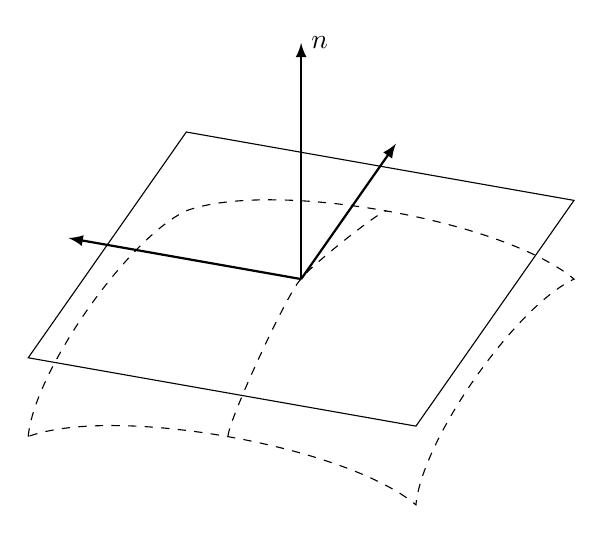
\begin{tikzpicture}[x={(170:1cm)},y={(55:.7cm)},z={(90:1cm)}, >=latex]
  \draw (2.5,-2.5,0) -- (2.5,2.5,0) -- (-2.5,2.5,0) -- (-2.5,-2.5,0) -- cycle;
  \draw[dashed,looseness=.6] (2.5,-2.5,-1) to[bend left] (2.5,2.5,-1) to[bend left] coordinate (mp) (-2.5,2.5,-1) to[bend right] (-2.5,-2.5,-1) to[bend right] coordinate (mm) (2.5,-2.5,-1) -- cycle;
  \draw[dashed,looseness=.2] (mm) to[bend left] (0,0,0) to[bend left] (mp);
  % \path[looseness=.2] (mm) to[bend left] node[pos=.2,pin={[pin distance=1cm,pin edge={solid,<-}]below right:$\gamma$}] {} (0,0,0);

  \draw[->, thick] (0,0,0) -- (3,0,0); % node[left] {$N\times\dot{\gamma}$};
  \draw[->, thick] (0,0,0) -- (0,3,0); % node[above right] {$\dot{\gamma}$};
  \draw[->, thick] (0,0,0) -- (0,0,3) node[right] {$n$};
  % \draw[dotted] (0,0,2) -- (1,0,2) -- (1,0,0);
  % \draw[->] (0,0,0) -- coordinate[pos=.3] (psi) (1,0,2); % node[above left] {$\ddot{\gamma}$};
  % \node[left] at (0,0,1.5) {$\kappa_n$};
  % \node[above] at (.5,0,0) {$\kappa_g$};
  % \draw (0,0,.8) to[out=170,in=55] node[above,fill=white,inner sep=1pt,outer sep=2pt] {$\psi$} (psi);
\end{tikzpicture}
\end{center}
\end{itemize}
\end{frame}

\begin{frame}[label={sec:org984931d}]{Forces}
\begin{itemize}
\item Normal forces \(\rightarrow\) same direction as surface

\item Shear forces \(\rightarrow\) perpendicular to surface direction
\end{itemize}
\end{frame}

\begin{frame}[label={sec:org9a573bd}]{Moments}
\begin{itemize}
\item Follow right-hand rule.

\item Torsional moments: same direction as surface

\item Bending moments: perpendicular to surface direction
\end{itemize}
\end{frame}

\begin{frame}[label={sec:org9236b00}]{The Singularity Equation (for this class)}
\begin{itemize}
\item Equilibrium equation
\end{itemize}

\[\sum F = 0\]
\[\sum M = 0\]
\end{frame}

\begin{frame}[label={sec:org7e46fb2}]{Engineering Statics}
\begin{itemize}
\item We will be trying to determine stresses and deformation of things

\item Need to find internal load at any point/surface

\item Method of sections
\end{itemize}
\end{frame}

\begin{frame}[label={sec:org17608de}]{Method of sections}
\begin{itemize}
\item Use free body diagram to determine internal forces/moments on surface
at any point

\item What if there are too loads/chages all at once

\item Principle of Superposition
\end{itemize}
\end{frame}

\begin{frame}[label={sec:org7e711b5}]{Principle of Superposition}
\begin{itemize}
\item Split the loads/changes

\item Determine individual response

\item Add the responses up
\end{itemize}
\end{frame}

\begin{frame}[label={sec:orgaa22efa}]{Review of High School Physics}
\begin{itemize}
\item Normal Stresses: same direction as surface

\item Shear stresses: perpendicular to surface direction
\end{itemize}
\end{frame}

\begin{frame}[label={sec:org04458e7}]{Normal Stresses}
\[\sigma = \frac{F_{normal}}{A}\]

\begin{center}
\includegraphics[height=0.7\textheight]{./pictures/normal-stress.png}
\end{center}
\end{frame}

\begin{frame}[label={sec:org5fba297}]{Shear Stresses}
\[\tau = \frac{F_{shear}}{A}\]

\includegraphics[width=\textwidth]{./pictures/shear-stress.png}
\end{frame}

\begin{frame}[label={sec:org6fe7099}]{Allowable Stresses}
\begin{itemize}
\item Real design needs to take care of uncertainties: materials,
conditions, loads, \ldots{}

\item Use \(\sigma_{allow}\) and \(\tau_{allow}\) instead
\end{itemize}

\begin{align*}
  \sigma_{allow} &= \frac{\sigma_{f}}{N_{s}} \\
  \tau_{allow} &= \frac{\tau_{f}}{N_{s}}
\end{align*}
\end{frame}

\begin{frame}[label={sec:org07c9a5a}]{Safety Factors, \(N_{s}\)}
\begin{itemize}
\item \(N_{s}\) is called the \emph{safety factor}

\item \(N_{s} \geqslant\) 1 always

\item Why? Is there an upper limit to \(N_{s}\)?
\end{itemize}
\end{frame}

\begin{frame}[label={sec:org40ee555}]{Example: Design with Safety Factor}
\begin{itemize}
\item We need a steel rod that will take the load of 20 kN with a safety
factor of 2. The steel rod has the maximum yield strength of 300 MPa.
Determine the required diameter of the rod.
\end{itemize}

\begin{align*}
    \sigma_{allow} &= \frac{F}{\pi r^{2}} = \frac{\sigma_{f}}{N_{s}} \\
    \frac{20000}{\pi r^{2}} &= \frac{300 \times 10^{6}}{2} \\
    r^{2} &= 4.24 \times 10^{-5} \\
    r &= 7.98 \times 10^{-3} \text{ m}
\end{align*}
\end{frame}

\begin{frame}[label={sec:org2ac1769}]{St. Venant's Principle}
\begin{center}
\includegraphics[width=.9\linewidth]{pictures/st-venant.png}
\end{center}

\begin{itemize}
\item Far enough away from load, stresses follow theoretical values
\end{itemize}
\end{frame}

\begin{frame}[label={sec:org08aa871}]{Normal Strain}
\begin{itemize}
\item Strain from lengthening or shortening of material
\end{itemize}

\[\varepsilon = \frac{\delta}{L}\]

\begin{figure}[h]
  \centering
  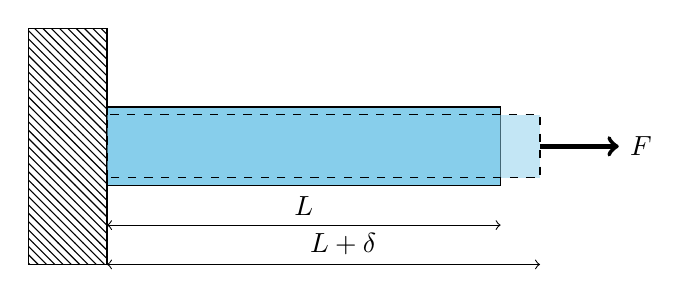
\begin{tikzpicture}
    \draw[pattern=north west lines] (-1,-1) rectangle (0,2);
    \draw[fill=SkyBlue] (0,0) rectangle (5,1);
    \draw[fill=SkyBlue, fill opacity=0.5, dashed] (0,0.1) rectangle (5.5,0.9);
    \draw[->,ultra thick] (5.5,0.5) -- (6.5,0.5) node[right]{$F$};
    \draw[<->] (0,-0.5) -- (2.5,-0.5) node[above]{$L$} -- (5,-0.5);
    \draw[<->] (0,-1) -- (3,-1) node[above]{$L + \delta$} -- (5.5,-1);
  \end{tikzpicture}
\end{figure}
\end{frame}

\begin{frame}[label={sec:orgcb317c7}]{Example: Ballooon}
\begin{itemize}
\item Air filled balloon with original radius \(r_1\) is pressurized until
its radius becomes \(r_2\). What is its strain?
\end{itemize}

\begin{center}
\includegraphics[height=0.6\textheight]{pictures/balloon-example.pdf}
\end{center}
\end{frame}

\begin{frame}[label={sec:org692b228}]{Shear Strain}
\begin{itemize}
\item Change in angular orientation of material
\end{itemize}

\[\gamma = \frac{\pi}{2} - \theta_f\]

\begin{figure}[h]
  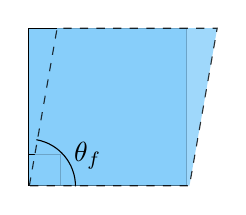
\begin{tikzpicture}
    \node [draw, fill=LightSkyBlue, minimum height=2cm, minimum width=2cm](base){};
    \node at (base.south west) [draw, minimum height=4mm, minimum width=4mm, anchor=south west]{};
    \node at (base.south west)[anchor=south west, xshift=2mm, draw, dashed, trapezium, trapezium left angle=80, trapezium right angle=100, fill=LightSkyBlue, opacity=0.8, minimum height=2cm, inner xsep=2.8]{};
    \draw (base.south west) ++ (0:0.6) arc (0:80:0.6) node[midway, right]{$\theta_{f}$};
  \end{tikzpicture}
\end{figure}
\end{frame}

\begin{frame}[label={sec:org950226d}]{Hooke's Law}
\begin{itemize}
\item How are stresses and strains related?

\item Normal stress-strain
\end{itemize}

\[\sigma = E \varepsilon\]

\begin{itemize}
\item Shear stress-strain
\end{itemize}

\[\tau = G \gamma\]

\begin{itemize}
\item \(E\) is Young's modulus or modulus of elasticity

\item \(G\) is shear modulus
\end{itemize}
\end{frame}

\begin{frame}[label={sec:orgb4a73dd}]{Material Behavior}
\begin{itemize}
\item Most engineering materials have two regions

\begin{itemize}
\item Elastic behavior: deformation is reversible

\item Plastic behavior: deformation is permanent
\end{itemize}
\end{itemize}
\end{frame}

\begin{frame}[label={sec:org7ca4627}]{Material Property Testing}
\begin{itemize}
\item Tensile Test: testing for material response
\end{itemize}

\begin{center}
\includegraphics[height=0.6\textheight]{./pictures/tensile-test-with-quattro.png}
\end{center}
\end{frame}

\begin{frame}[label={sec:orgc4c54be}]{Material Types}
\begin{center}
\includegraphics[height=0.6\textheight]{pictures/material-type-behavior.pdf}
\end{center}
\end{frame}

\begin{frame}[label={sec:org7f5fcd3}]{Stress - Strain Diagram: Ductile}
\footnotesize
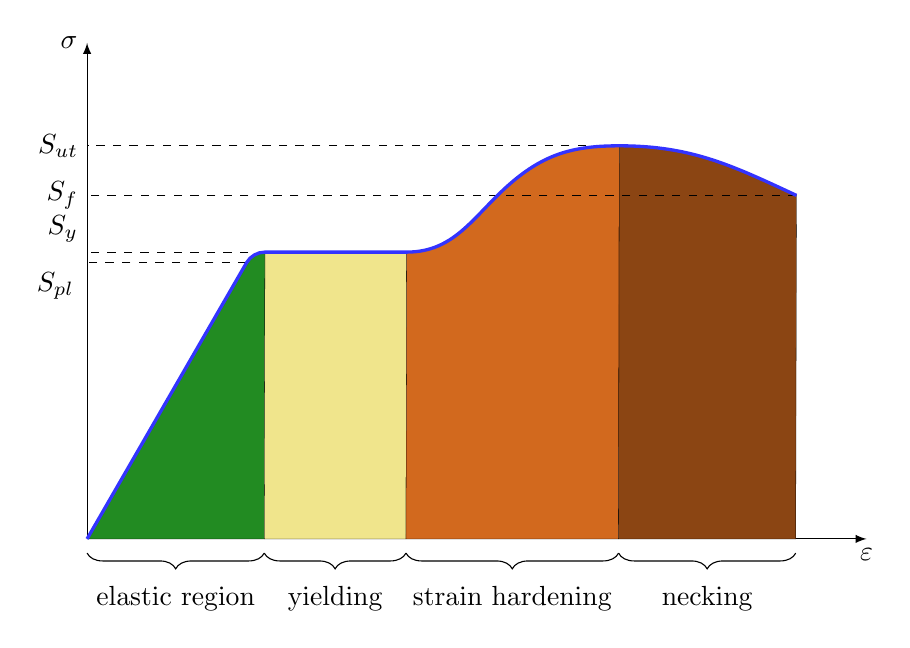
\begin{tikzpicture}[scale=0.9,>=latex]
  % axes
  \draw [<->] (0,7) node[left]{$\sigma$} --++ (-90:7) node(O){} --++ (0:11) node[below]{$\varepsilon$};
  % braces
  \draw [decorate, decoration={brace, mirror, amplitude=2mm}] (O.center) ++ (-90:0.2) --++ (0:2.5) node(B){} node[midway, below, yshift=-3mm]{elastic region};
  \draw [decorate, decoration={brace, mirror, amplitude=2mm}] (B.center) --++ (0:2) node(C){} node[midway, below, yshift=-3mm]{yielding};
  \draw [decorate, decoration={brace, mirror, amplitude=2mm}] (C.center) --++ (0:3) node(D){} node[midway, below, yshift=-3mm]{strain hardening};
  \draw [decorate, decoration={brace, mirror, amplitude=2mm}] (D.center) --++ (0:2.5) node(E){} node[midway, below, yshift=-3mm]{necking};
  % area under curve
  \draw [ultra thin, fill=ForestGreen] (B.center) ++ (90:0.2) node(F){} -- (O.center) --++ (60:4.5) node(pl){} arc (150:90:0.3) node(G){} -- cycle;
  \draw [ultra thin, fill=Khaki] (C.center) ++ (90:0.2) node(H){} -- (F.center) -- (G.center) --++ (0:2) node(I){} -- cycle;
  \draw [ultra thin, fill=Chocolate] (D.center) ++ (90:0.2) node(J){} -- (H.center) -- (I.center) to [out=0, in=-140] ++(1.5,1) to [out=40,in=180] ++(1.5,0.5) node(K){} -- cycle;
  \draw [ultra thin, fill=SaddleBrown] (E.center) ++ (90:0.2) node(L){} -- (J.center) -- (K.center) to [out=0, in=155] ++(2.5,-0.7) node(M){} -- cycle;
  % stress indicators
  \draw [dashed] (pl.center) -- +(180:2.3) node[below left]{$S_{pl}$};
  \draw [dashed] (G.center) -- +(180:2.5) node[above left]{$S_{y}$};
  \draw [dashed] (K.center) -- +(180:7.5) node[left]{$S_{ut}$};
  \draw [dashed] (M.center) -- +(180:10) node[left]{$S_{f}$};
  % actual curve
  \draw [very thick, Blue!80](O.center) -- (pl.center) arc (150:90:0.3) -- (I.center) to [out=0, in=-140] ++(1.5,1) to [out=40,in=180] ++(1.5,0.5) to [out=0, in=155] ++(2.5,-0.7);
\end{tikzpicture}
\end{frame}

\begin{frame}[label={sec:org7973874}]{Elastic Region}
\begin{itemize}
\item Deformation is reversible \(\rightarrow\) object returns to original
shape once load is removed

\item Most designed parts are meant to operate in this region
\end{itemize}
\end{frame}

\begin{frame}[label={sec:orgbc29381}]{Yield}
\begin{itemize}
\item Transition from elastic to plastic deformation \(\sim\) material
failure

\item Difficult to specify exact location

\item Definition can vary

\begin{enumerate}
\item proportionality limit

\item elastic limit

\item offset yield point (0.2\% rule)
\end{enumerate}
\end{itemize}
\end{frame}

\begin{frame}[label={sec:orgc757106}]{Strain Hardening}
\begin{itemize}
\item Deformation in materials cause temperary hardness increases

\item Material can take additional stress because of this
\end{itemize}
\end{frame}

\begin{frame}[label={sec:org2c8a083}]{Necking}
\begin{columns}
\begin{column}{0.5\columnwidth}
\begin{center}
\includegraphics[width=.9\linewidth]{pictures/necking.png}
\end{center}
\end{column}

\begin{column}{0.5\columnwidth}
\begin{itemize}
\item Final phase of plastic deformation before failure

\item Cross-sectional area decreases \(\rightarrow\) increased stress
\end{itemize}
\end{column}
\end{columns}
\end{frame}

\begin{frame}[label={sec:org7996e8d}]{Strain Energy}
\begin{itemize}
\item Energy stored in deformed body

\item Assumed equal to work done by external loadings

\begin{align*}
  u &= \frac{1}{2}\sigma\varepsilon \\
    &= \frac{1}{2}\frac{\sigma^2}{E}
\end{align*}

\item Area under \(\sigma-\varepsilon\) curve

\item Important to material strength under impact loading
\end{itemize}
\end{frame}

\begin{frame}[label={sec:org337a723}]{Modulus of Resilience}
\begin{figure}[h]
  \centering
  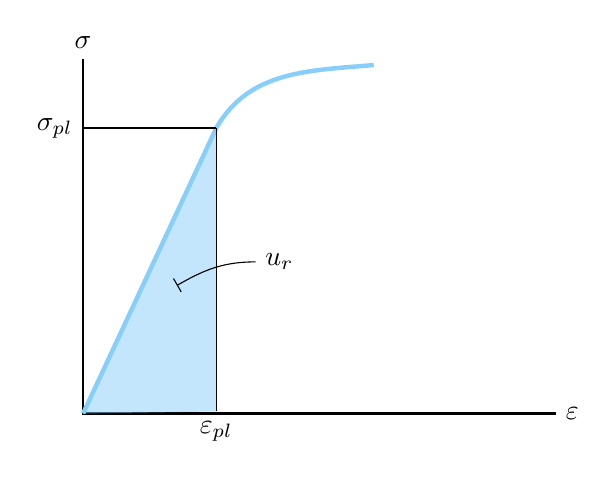
\begin{tikzpicture}
    \draw [thick] (0,4.5) node[above]{$\sigma$} --++ (-90:4.5) --++ (0:6) node[right]{$\varepsilon$};
    \draw [ultra thick, LightSkyBlue] (0,0) --++ (65:4) node(pl){} to[out=60, in=185] +(2,0.8);
    \path[fill=LightSkyBlue, fill opacity=0.5] (0,0) -- (pl.center) --++ (-90:3.6) -- cycle;
    \draw [|-] (pl) ++ (-0.5,-2) to[out=30,in=180] +(1,0.3) node[right]{$u_r$};
    \draw (pl.center) --++ (-90:3.6) node[below]{$\varepsilon_{pl}$};
    \draw (pl.center) --++ (180:1.7) node[left]{$\sigma_{pl}$};
  \end{tikzpicture}
\end{figure}

\begin{itemize}
\item Amount of energy to permanently deform body
\end{itemize}
\end{frame}

\begin{frame}[label={sec:org2cfc441}]{Modulus of Toughness}
\begin{figure}[h]
  \centering
  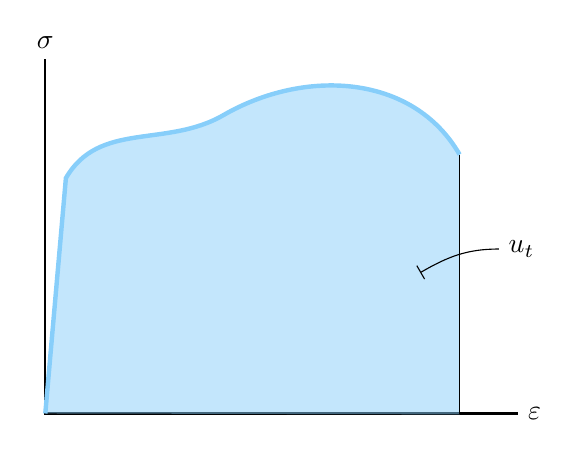
\begin{tikzpicture}
    \draw [thick] (0,4.5) node[above]{$\sigma$} --++ (-90:4.5) --++ (0:6) node[right]{$\varepsilon$};
    \draw [ultra thick, LightSkyBlue] (0,0) --++ (85:3) node(pl){} to[out=60, in=210] ++(2,0.8) to[out=30,in=120] ++(3,-0.5);
    \path[fill=LightSkyBlue, fill opacity=0.5] (0,0) -- (pl.center) to[out=60, in=210] ++(2,0.8) to[out=30,in=120] ++(3,-0.5) node(ut){} --++ (-90:3.30) -- cycle;
    \draw (ut.center) --++ (-90:3.30);
    \draw [|-] (ut) ++ (-0.5,-1.5) to[out=30,in=180] +(1,0.3) node[right]{$u_t$};
  \end{tikzpicture}
\end{figure}

\begin{itemize}
\item Amount of energy to fracture body
\end{itemize}
\end{frame}

\begin{frame}[label={sec:org607f94e}]{Shear Stress-Strain Relationship}
\begin{figure}[h]
  \centering
  \begin{tikzpicture}[>=latex, scale=1.2]
    % axes
    \draw [<->] (0,5) node[left]{$\sigma$} --++ (-90:5) node(O){} --++ (0:5) node[below]{$\varepsilon$};
    % curve
    \draw [very thick, Blue!80](O.center) --++ (1,2.5) node(pl){} to[out=60, in=180] ++ (2,1) node(u){} to[out=0, in=145] ++ (1.5,-0.4) node(f){};
    \draw [dashed] (pl.center) --++ (180:1) node[left]{$\tau_{pl}$};
    \draw [dashed] (u.center) --++ (180:3) node[left]{$\tau_{u}$};
    \draw [dashed] (f.center) --++ (180:4.5) node[left]{$\tau_{f}$};
  \end{tikzpicture}
\end{figure}
\end{frame}

\begin{frame}[label={sec:org19ab7f8}]{Thermal Strain}
\begin{itemize}
\item Change in temperature causes material deformation

\begin{itemize}
\item material normally expands when heated and contracts when cooled
\end{itemize}

\item Definition in 1-D

\begin{align*}
  \alpha = \frac{1}{L} \frac{d L}{dT}
\end{align*}

\item \(\alpha\) is called the coefficient of thermal expansion (CTE)
\end{itemize}
\end{frame}

\begin{frame}[label={sec:org43175db}]{Properties of \(\alpha\)}
\begin{itemize}
\item \(\alpha\) is typically a function of \(T\)

\item For many engineering materials (solids), \(\alpha\) \(\sim\) constant
\end{itemize}

\[\delta = \int_0^L \alpha \Delta T dx\]

\begin{itemize}
\item For uniform temperature change
\end{itemize}

\[\delta = \alpha \Delta T L\]
\end{frame}

\begin{frame}[label={sec:orgfa53b39}]{Example: Heated Bar}
\begin{itemize}
\item If a beam has an original length of 2 m and initial \(T\) = 20 C

\item The beam is heated, after which the temperature along the beam is
\(T(x) = 20 x^2 + 10x + 30\) C. Beam has \(\alpha\) = 2.5
10\(^{\text{-6}}\)

\begin{itemize}
\item What is the deformation of the middle point of the beam?

\item What is the final length of the beam?
\end{itemize}
\end{itemize}
\end{frame}

\begin{frame}[label={sec:org23045e2}]{Poisson's Effect}
\begin{columns}
\begin{column}{0.5\columnwidth}
\begin{figure}
  \centering
  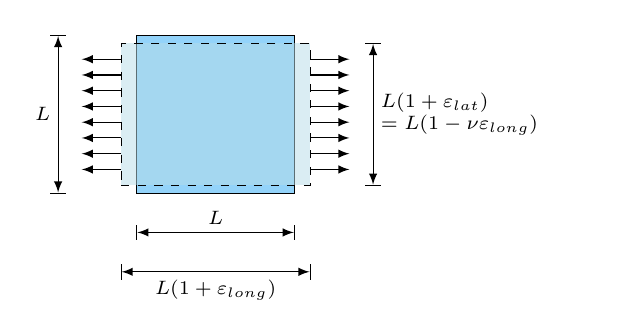
\begin{tikzpicture}[>=latex]
    \scriptsize
    \node [draw, rectangle, minimum height=2cm, minimum width=2cm, fill=LightSkyBlue!90, inner sep=0](A){};
    \node [draw, dashed, rectangle, minimum height=1.8cm, minimum width=2.4cm, fill=LightBlue!90, fill opacity=0.5, inner sep=0](B){};
    \foreach \x in {1,...,8} {
      \draw [->] (1.2, 0.9-0.2*\x) --++ (0:0.5);
      \draw [->] (-1.2, 0.9-0.2*\x) --++ (180:0.5);
    }

    \node at (A.west) [yshift=-1.5cm](C){};
    \node at (A.east) [yshift=-1.5cm](D){};

    \node at (B.west) [yshift=-2cm](E){};
    \node at (B.east) [yshift=-2cm](F){};

    \draw [|<->|] (C.center) -- (D.center) node[midway,above]{$L$};
    \draw [|<->|] (E.center) -- (F.center) node[midway,below]{$L(1+\varepsilon_{long})$};

    \node at (A.north) [xshift=-2cm](G){};
    \node at (A.south) [xshift=-2cm](H){};

    \node at (B.north) [xshift=2cm](I){};
    \node at (B.south) [xshift=2cm](J){};

    \draw [|<->|] (G.center) -- (H.center) node[midway,left]{$L$};
    \draw [|<->|] (I.center) -- (J.center) node[text width=2.7cm,midway,right]{$L(1+\varepsilon_{lat})$ \\
      $= L(1-\nu\varepsilon_{long})$};
      \end{tikzpicture}
\end{figure}
\end{column}

\begin{column}{0.5\columnwidth}
\begin{itemize}
\item Material's lateral contraction (extension) under longitudinal tensile
(compressive) load
\end{itemize}

\[\nu = - \frac{\varepsilon_{lat}}{\varepsilon_{long}}\]

\begin{itemize}
\item \(\nu\) is called \emph{Poisson's ratio}
\end{itemize}
\end{column}
\end{columns}
\end{frame}

\begin{frame}[label={sec:org7d237b5}]{Poisson's Ratio Range}
\begin{columns}
\begin{column}{0.5\columnwidth}
\footnotesize
\begin{center}
\begin{tabular}{lr}
\toprule
Material & Poisson's ratio\\\empty
\midrule
rubber & 0.4999\\\empty
gold & 0.42--0.44\\\empty
saturated clay & 0.40--0.49\\\empty
magnesium & 0.252-0.289\\\empty
titanium & 0.265-0.34\\\empty
copper & 0.33\\\empty
aluminium-alloy & 0.32\\\empty
clay & 0.30--0.45\\\empty
stainless steel & 0.30--0.31\\\empty
steel & 0.27--0.30\\\empty
cast iron & 0.21--0.26\\\empty
sand & 0.20--0.45\\\empty
concrete & 0.1-0.2\\\empty
glass & 0.18--0.3\\\empty
foam & 0.10--0.50\\\empty
cork & 0\\\empty
\bottomrule
\end{tabular}
\end{center}
\end{column}

\begin{column}{0.5\columnwidth}
\begin{itemize}
\item Usual engineering materials have \(0 \leqslant \nu \leqslant 0.5\)
\end{itemize}
\end{column}
\end{columns}
\end{frame}

\begin{frame}[label={sec:orgc3b1431}]{Auxetic Material}
\begin{columns}
\begin{column}{0.5\columnwidth}
\begin{itemize}
\item Materials that exhibit negative Poisson's ratios

\item How is that possible?

\item Rely on material microstructure

\item Useful in many design situations
\end{itemize}
\end{column}

\begin{column}{0.5\columnwidth}
\begin{center}
\begin{center}
\includegraphics[width=.9\linewidth]{./pictures/auxetic-footwear.jpg}
\end{center}
\end{center}
\end{column}
\end{columns}
\end{frame}

\begin{frame}[label={sec:orgf31df22}]{Mechanical Strains vs Thermal Strains}
\begin{itemize}
\item Strains caused by load vs temperature change

\item Mechanical strains: normal strains + lateral strains from Poisson's
effect

\item Thermal strains: strains in all direction, \emph{no} Poisson's effect.

\item \(\varepsilon_{\text{total}} = \varepsilon_{\text{mech}} + \varepsilon_{\text{therm}}\)
(mind the signs)
\end{itemize}
\end{frame}

\begin{frame}[label={sec:org889ef94}]{Mech vs Therm Strains Example}
A circular cross-sectioned steel bar with
radius \(r\) = 1 cm and length \(L\) = 2 m is stretched along its length
by a stress of 100 MPa. If the steel has \(E\) = 210 GPa, \(\nu\) = 0.3,
and \(\alpha\) = 16 \(\times\) 10\(^{-6}\)/\(^{\circ}C\), how much
temperature change does it need to return to its original volume?
\end{frame}

\begin{frame}[label={sec:org172daef}]{Solution: Mech vs Therm Strains}
Match before and after volumes

before:

\begin{align*}
    V_{0} &= \pi r^{2} l
\end{align*}

after:

\begin{align*}
    l_{1} &= l \left( 1 + \frac{\sigma}{E} + \alpha \Delta T \right) \\
          %&= 2 \left( 1 + \frac{1 \times 10^{6}}{210 \times 10^{9}}  + 16 \times 10^{-6}\Delta T \right) \\
    r_{1} &= r \left( 1 - \nu \frac{\sigma}{E} + \alpha \Delta T \right) \\
          %&= 0.01 \left( 1 - 0.3 \frac{1 \times 10^{6}}{210 \times 10^{9}} + 16 \times 10^{-6} \Delta T \right)
\end{align*}
\end{frame}

\begin{frame}[label={sec:orgc38f22f}]{Solution: Mech vs Therm Strains}
Set \(V_0 = V_{1}\)

\begin{align*}
    \pi r^{2} l &= \pi r^{2}\left(1 - \nu \frac{\sigma}{E} + \alpha \Delta T \right)^{2} l\left( 1 + \frac{\sigma}{E} + \alpha \Delta T \right) \\
\end{align*}

Keep only first-order terms:

\begin{align*}
    0 &= \frac{\sigma}{E} -\nu \frac{\sigma}{E} -\nu \frac{\sigma}{E} + 2\alpha \Delta T + \alpha \Delta T \\
    \Delta T &= \frac{-\sigma(1 - 2 \nu)}{3 \alpha E} \\
      &= -3.97 \text{ C}
\end{align*}
\end{frame}

\begin{frame}[label={sec:org9c12122}]{Thermal Stress}
\begin{itemize}
\item Stress in a cooled/heated material constrained from deforming freely
\end{itemize}
\end{frame}

\begin{frame}[label={sec:orga697cfa}]{Example: Hot Bar / Cool Bar}
\begin{itemize}
\item A metal bar is constrained between two walls the same distance as the
beam's length, how would you change the temperature so that the beam
is \ldots{}

\begin{itemize}
\item in tension?

\item in compression?
\end{itemize}

\item We can intuit the \emph{direction} of temperature change (up or down),
\emph{but} not yet its magnitude (how much)

\item We will learn that soon enough \ldots{}
\end{itemize}
\end{frame}
\end{document}